% Copyright 2004 by Till Tantau <tantau@users.sourceforge.net>.
%
% In principle, this file can be redistributed and/or modified under
% the terms of the GNU Public License, version 2.
%
% However, this file is supposed to be a template to be modified
% for your own needs. For this reason, if you use this file as a
% template and not specifically distribute it as part of a another
% package/program, I grant the extra permission to freely copy and
% modify this file as you see fit and even to delete this copyright
% notice. 

\documentclass{beamer}
% Replace the \documentclass declaration above
% with the following two lines to typeset your 
% lecture notes as a handout:
%\documentclass{article}
%\usepackage{beamerarticle}

\usepackage{graphicx}
\usepackage[utf8]{inputenc}
 
\graphicspath{ {img/} }


% There are many different themes available for Beamer. A comprehensive
% list with examples is given here:
% http://deic.uab.es/~iblanes/beamer_gallery/index_by_theme.html
% You can uncomment the themes below if you would like to use a different
% one:
%\usetheme{AnnArbor}
%\usetheme{Antibes}
%\usetheme{Bergen}
%\usetheme{Berkeley}
%\usetheme{Berlin}
%\usetheme{Boadilla}
%\usetheme{boxes}
%\usetheme{CambridgeUS}
%\usetheme{Copenhagen}
%\usetheme{Darmstadt}
%\usetheme{default}
%\usetheme{Frankfurt}
%\usetheme{Goettingen}
%\usetheme{Hannover}
%\usetheme{Ilmenau}
%\usetheme{JuanLesPins}
%\usetheme{Luebeck}
%\usetheme{Madrid}
%\usetheme{Malmoe}
%\usetheme{Marburg}
%\usetheme{Montpellier}
%\usetheme{PaloAlto}
%\usetheme{Pittsburgh}
%\usetheme{Rochester}
%\usetheme{Singapore}
%\usetheme{Szeged}
\usetheme{Warsaw}

\title{Programming with NodeJS}

% A subtitle is optional and this may be deleted
\subtitle{Lesson 1: Setting up, the event loop and callback functions}

%\author{F.~Author\inst{1} \and S.~Another\inst{2}}
% - Give the names in the same order as the appear in the paper.
% - Use the \inst{?} command only if the authors have different
%   affiliation.

%\institute[Universities of Somewhere and Elsewhere] % (optional, but mostly needed)
%{
%  \inst{1}%
%  Department of Computer Science\\
%  University of Somewhere
%  \and
%  \inst{2}%
%  Department of Theoretical Philosophy\\
%  University of Elsewhere}
% - Use the \inst command only if there are several affiliations.
% - Keep it simple, no one is interested in your street address.

\date{Febuary 7th, 2017}
% - Either use conference name or its abbreviation.
% - Not really informative to the audience, more for people (including
%   yourself) who are reading the slides online

\subject{NodeJS Lessons}
% This is only inserted into the PDF information catalog. Can be left
% out. 

% If you have a file called "university-logo-filename.xxx", where xxx
% is a graphic format that can be processed by latex or pdflatex,
% resp., then you can add a logo as follows:

% \pgfdeclareimage[height=0.5cm]{university-logo}{university-logo-filename}
% \logo{\pgfuseimage{university-logo}}

% Delete this, if you do not want the table of contents to pop up at
% the beginning of each subsection:
%\AtBeginSubsection[]
%{
%  \begin{frame}<beamer>{Outline}
%    \tableofcontents[currentsection,currentsubsection]
%  \end{frame}
%}

% Let's get started
\begin{document}

\begin{frame}
  \titlepage
\end{frame}

%\begin{frame}{Outline}
%  \tableofcontents
%  % You might wish to add the option [pausesections]
%\end{frame}

% Section and subsections will appear in the presentation overview
% and table of contents.
\section{Introduction}

\subsection{Setting up and basics}

\begin{frame}{What is NodeJS? What programming languages is it like?}
\pause
Previous series:\\
\pause
\textit{https://github.com/Casper-Oakley/python-lessons}\\
\pause
This series:\\
\pause
\textit{https://github.com/Casper-Oakley/nodejs-lessons}
\pause
\begin{figure}[h]
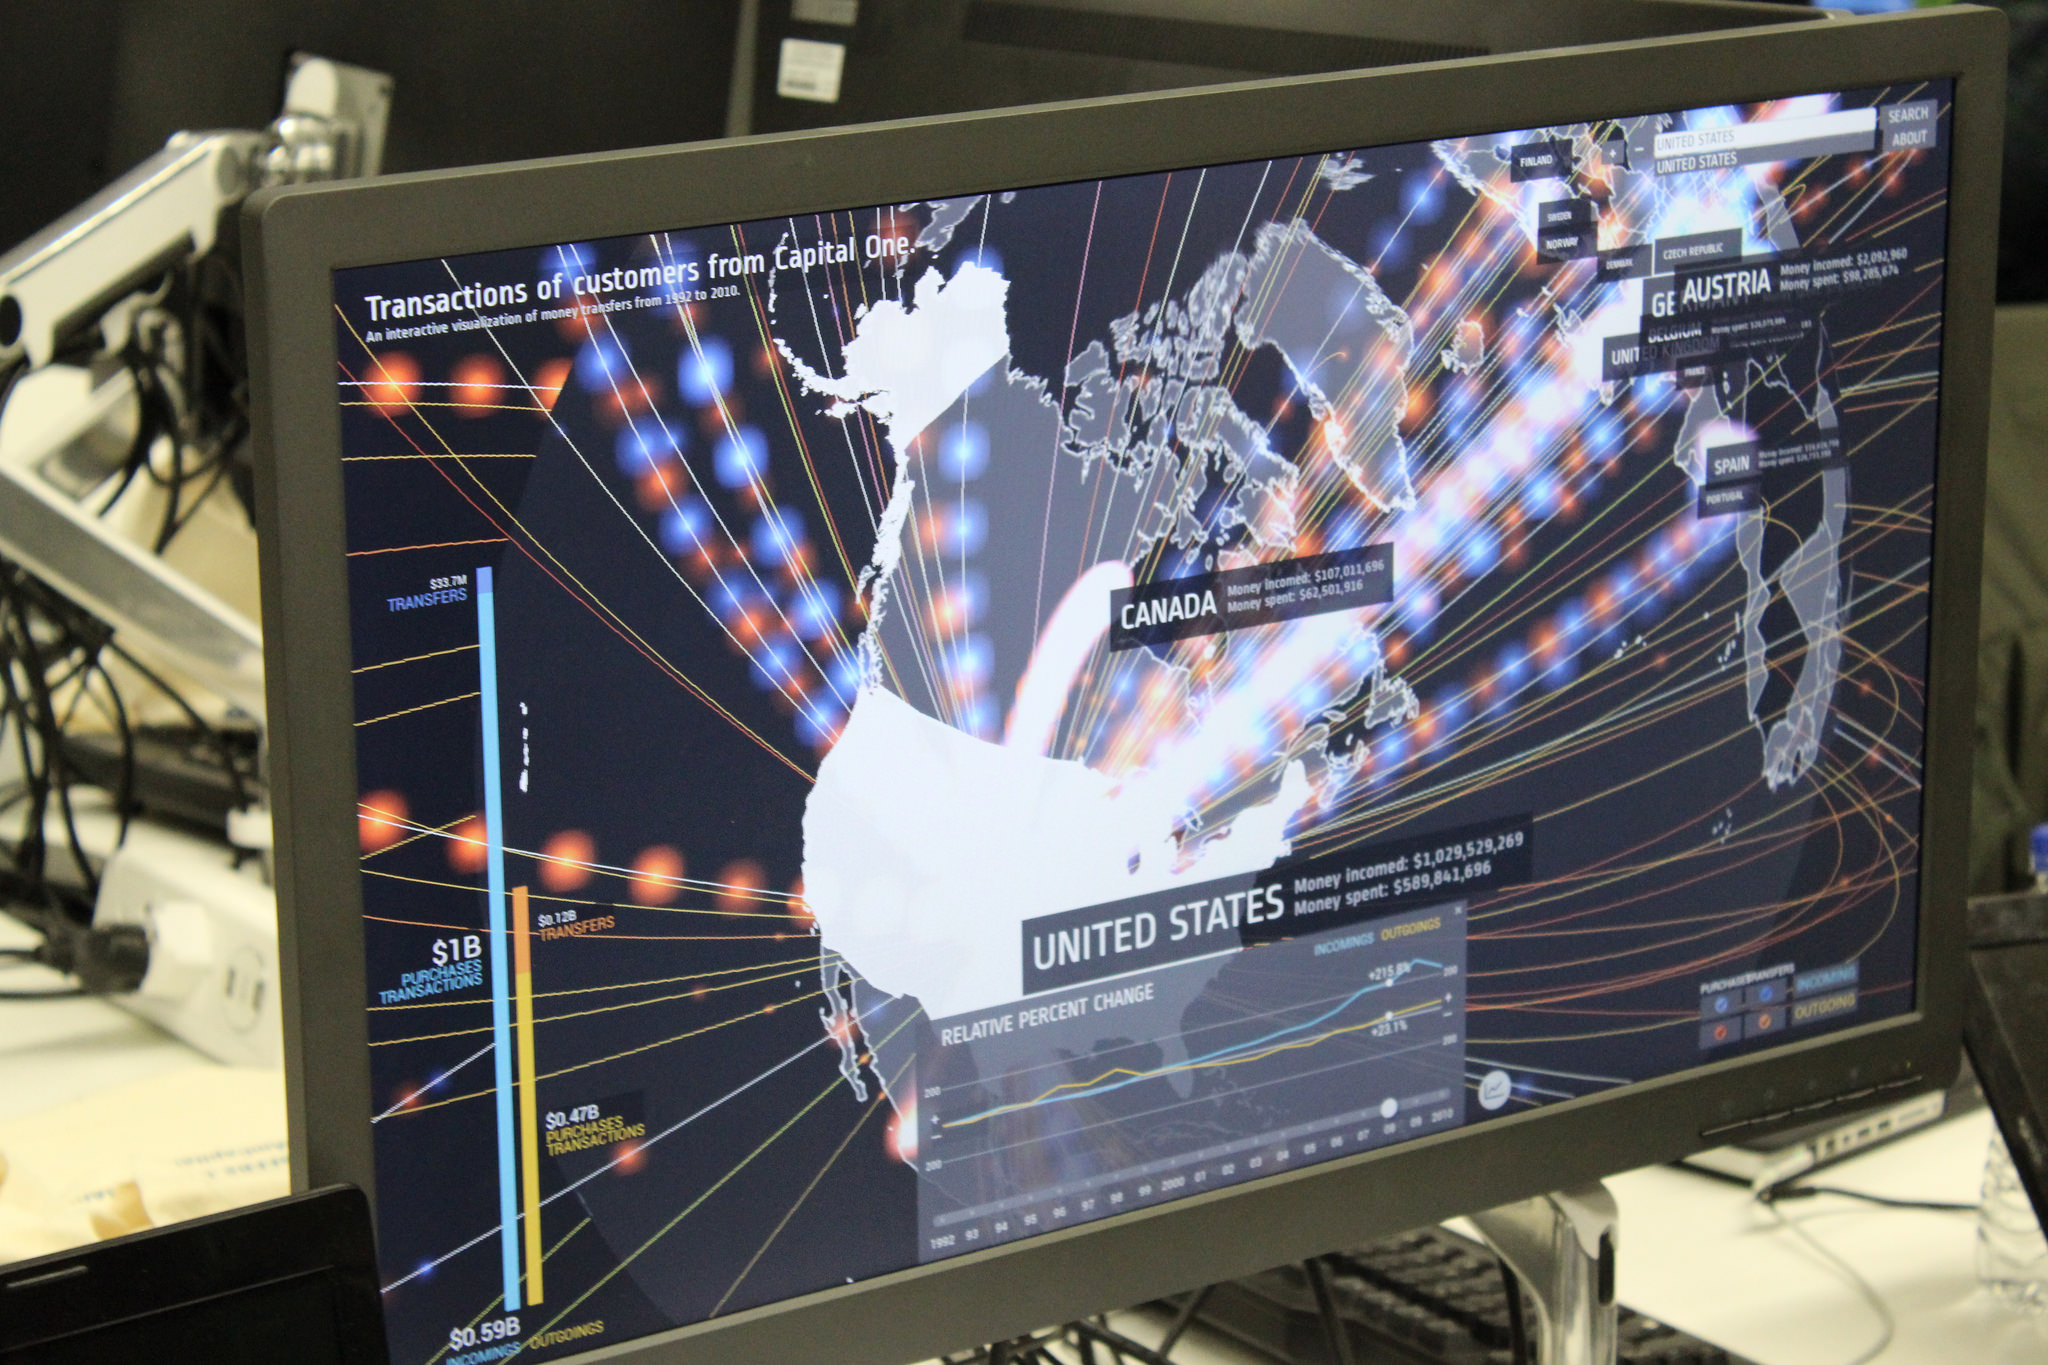
\includegraphics[width=0.4\textwidth]{wow}
\caption{Image curtosy of HackSocNotts}
\end{figure}
\end{frame}

\begin{frame}{Setting up your development environment}

We will be using  version: v6.9.5 (with npm version 3.10.10)

\begin{itemize}
  \item {
    Windows: \textbf{https://nodejs.org/en/download/}
  }
  \item {
    Mac OSX: \textbf{https://nodejs.org/en/download/}
  }
  \item {
    Linux: Either \textbf{sudo apt-get install nodejs} or \textbf{https://nodejs.org/en/download/}
  }
\end{itemize}

If at any time you get stuck, just stick your hand up.

\end{frame}

\begin{frame}{Setting up your development environment}
You will also need a text editor. The choice of text editor is up to what you feel most comfortable using.
\pause
Some options include:
\begin{itemize}
  \pause
  \item notepad++
  \pause
  \item Vim
  \pause
  \item GNU Emacs
  \pause
  \item atom \pause - Fun fact, this was actually written in part in NodeJS!
\end{itemize}
\end{frame}

% Placing a * after \section means it will not show in the
% outline or table of contents.
\section*{Hello, World!}

\begin{frame}{The basics of NodeJS}
NodeJS is an extremely powerful language developed on top of the V8 javascript engine, written by google.
\pause
It operates on a single thread, using an event loop to manage concurrency.
\pause
It has been found to be particularly strong in certain areas:
\pause
\begin{itemize}
  \item I/O bound applications \pause
  \item Data streaming applications\pause
  \item JSON APIs\pause
  \item As the backend in a MEAN stack web app \pause - This is the one we will focus on
\end{itemize}
\end{frame}

\begin{frame}{Running NodeJS code}

Two ways to run your NodeJS code:

\begin{itemize}
  \item Through the command line interpreter (the REPL)
  \item By putting your code into a file and executing the file
\end{itemize}

\pause
demo

\end{frame}


\begin{frame}{NPM: node package manager}

NodeJS's strengths lie mainly in it's ability to route information from places to other places, not to do heavy computation/store data/render stuff.
\pause
The Node Package Manager (NPM) sources all kinds of packages for NodeJS, each of which can be installed in one simple command!
\pause
\textit{https://www.npmjs.com/}

\end{frame}

\begin{frame}{That's all for tonight!}
  To summarise:
  \begin{itemize}
  \item We have installed Python and PyCharm
  \item We have learnt about variables and variable types
  \item We have learnt about printing and asking for input from the user
  \item We have made a sweet ass calculator!
  \end{itemize}
\end{frame}

\begin{frame}{For next week}
Source code plus lecture slides will be available online soon after the lesson.\\
If you are new to HackSocNotts, please join us on \textit{http://hacksocnotts.slack.com}.\\
If you have any questions, feel free to ask now or over slack.\\
\end{frame}

\end{document}


